\documentclass[a4paper,titlepage,twoside,12pt,leqno]{article}

\usepackage[]{fontspec}
\usepackage{xltxtra}
\usepackage[monogreek]{xgreek}

\newcommand{\en}[1]{\setlanguage{american}#1\setlanguage{monogreek}} % Για υφενώσεις στα αγγλικά

\defaultfontfeatures{Mapping=tex-text%, Scale=MatchLowercase}
} 

% Γραμματοσειρά
\setmainfont[Mapping=tex-text]{DejaVu Sans}


\usepackage{longtable} % για έναν μεγάλο πίνακα
\usepackage{graphicx, array, blindtext}

\title{Αναλυτικό εγχειρίδιο αναφοράς για το ηλεκτρονικό θεματικό πάρκο σε μεσαιωνική καστροπολιτεία}
\author{Αναγνωστόπουλος Βασίλης-Θάνος, Κατσής Γιώργος}
\date{}

\begin{document}

\maketitle
\tableofcontents
\listoffigures
\listoftables
\newpage

\section{Εισαγωγή}

%Στα εγχειρίδια αυτά παρουσιάζεται η σύνταξη όλων των εντολών του προγράμματος. Σε αυτά τα εγχειρίδια ανατρέχει ένας χρήστης για να βρει την σύνταξη της οποιασδήποτε εντολής. Ο στόχος των εγχειριδίων αυτών είναι να καλύψουν πλήρως τη λειτουργία ενός προγράμματος και όχι να εκπαιδεύσουν το χρήστη. Αυτά τα εγχειρίδια χρησιμεύουν σε όλους τους χρήστες, είτε αυτοί είναι καινούριοι είτε παλαιότεροι οπότε γνωρίζουν λίγο πολύ τη λειτουργία του προγράμματος.

\emph{Σημείωση: Τα κείμενα το οποία είναι γραμμένα σε πλάγια γραφή (όπως και το συγκεκριμένο) είναι σημειώσεις, οι οποίες θα απομακρυνθούν από το τελικό κείμενο, αλλά αυτή την στιγμή υποδηλώνουν εργασίες οι οποίες δεν μπορούν να ολοκληρωθούν χωρίς να αναπτυχθεί ο κώδικας της εφαρμογής ή για κάποιο άλλο παρεμφερή λόγο.\\}

Το συγκεκριμένο πρόγραμμα προορίζεται για την αλληλεπίδραση των ενοίκων του μεσαιωνικού κάστροδιαμερίσματος με τις διάφορες συσκευές και υπηρεσίες που διαθέτει το διαμέρισμα του και η καστοπολιτεία. Συγκεκριμένα μέσα αυτού του προγράμματος μπορείτε να διαχειριστεί τις παρακάτω συσκευές:

\begin{itemize}
\item την πόρτα του διαμερίσματος του (βλέπε σελ. \ref{pisina})
\item Πισίνα (βλέπε σελ. \ref{pisina})
\item Να βάλουμε και άλλες συσκευές.
\end{itemize}

\emph{Σημείωση: Εδώ θα μπει η πλήρης λίστα με τις συσκευές που μπορεί να αλληλεπιδράσει ο χρήστης καθώς και που βρίσκονται.}

\section{Πλοήγηση στην εφαρμογή}

\emph{Σημείωση: Τα εγχειρίδια προτιμήθηκε να γραφούν σε λιγότερη επίσημη γλώσσα. Η επιλογή αυτή είναι λάθος; Επίσης τί κεφάλαια να περιλαμβάνονται σε αυτό το εγχειρίδιο;\\}

Η πρώτη οθόνη της εφαρμογής είναι για την επιλογή του κατάλληλου μενού για την αλληλεπίδραση με την καστροπολιτεία. Στα δεξιά του παραθύρου φαίνονται σημαίες από χώρες που πατώντας και πατώντας κάποια σημαία αλλάζει η γλώσσα των μηνυμάτων που εμφανίζονται στην εφαρμογή.

Στα αριστερά της εφαρμογής φαίνονται τα εικονίδια επιλογών καθώς και ένα μικρό κείμενο το οποίο επεξηγεί τί κάνει το καθένα (βλ. σχήμα \ref{fig:menu:general})

\begin{figure}
\begin{center}
\resizebox*{10.5cm}{!}{
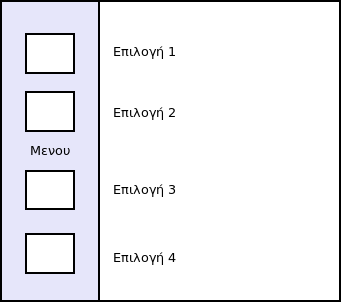
\includegraphics{images/menu.png}}
\caption{Το γενικό μενού (σε αφηρημένη μορφή).}
\label{fig:menu:general}
\end{center}
\end{figure}

Στον πίνακα \ref{table:icons} φαίνονται αναλυτικά τα εικονίδια καθώς και το τί κάνουν.

\begin{table}
\begin{center}
  \begin{tabular}{|m{0.20\textwidth}|m{0.70\textwidth}|}
    \hline
     
     \resizebox*{!}{0.20\textwidth}{
     \rule{0.4\textwidth}{0.4\textwidth}}

     & κείμενο για το σχήμα. \\ \hline



    \hline
  \end{tabular}
\caption{Τα εικονίδια της εφαρμογής}
\label{table:icons}
\end{center}
\end{table}

\emph{\\Σημείωση: Εδώ θα μπει πίνακας για να τα επεξηγεί, αλλά από την στιγμή που δεν έχει αποφασιστεί ακόμα το σχήμα τους και η λειτουργικότητα τους παραλείφθηκαν.\\}

Όταν πατηθεί κάποιο εικονίδιο τότε μεταβαίνουμε σε ένα νέο παράθυρο το οποίο αλλάζει ανάλογα με την επιλογή, όμως το μενού με τα εικονίδια στα αριστερά θα παραμένει έτσι ώστε να είναι δυνατή η εναλλαγή μεταξύ των μενού γρήγορα να είμαστε υποχρεωμένοι να γυρίσουμε στην αρχική οθόνη.

\section{Παραγγελία αντικειμένων}
\label{paraggelia}

Σε αυτό το μενού μπορούμε να παραγγείλουμε προϊόντα από την καφετέρια-εστιατόριο της καστροπολιτείας μας. Για να εισέλθουμε σε αυτό το μενού θα πρέπει να πατήσουμε το εικονίδιο με τους (περιγραφή) από το κεντρικό μενού (βλ. σχήμα \ref{}).

\emph{\\Σημείωση: Επειδή ακόμα δεν έχουν αποσαφηνιστεί η λεπτομέρειες με τα εικονίδια αφέθηκαν κενά.\\}

\begin{figure}
\begin{center}
\resizebox*{10.5cm}{!}{
\rule{0.4\textwidth}{0.3\textwidth}}
\caption{Το εικονίδιου για την μετάβαση σε .....}
\label{fig:icon:}
\end{center}
\end{figure}

Αρχικά εμφανίζονται οι κατηγορίες των αντικειμένων των οποίων μπορούμε να αγοράσουμε από την καφετέρια-εστιατόριο της καστροπολιτείας μας (βλ. σχήμα \ref{})

\begin{figure}
\begin{center}
\resizebox*{10.5cm}{!}{
\rule{0.4\textwidth}{0.3\textwidth}}
\caption{Το εικονίδιου για την μετάβαση σε .....}
\label{fig:icon:}
\end{center}
\end{figure}

Επιλέγοντας μία κατηγορία "ανοίγουν" και εμφανίζονται τα προϊόντα σε αυτή την κατηγορία. Επιλέγοντας ένα από τα αντικείμενα ανοίγει μία νέα φόρμα που περιγράφει αναλυτικά το αντικείμενο (βλ. σχήμα \ref{}).

\begin{figure}
\begin{center}
\resizebox*{10.5cm}{!}{
\rule{0.4\textwidth}{0.3\textwidth}}
\caption{Το εικονίδιου για την μετάβαση σε .....}
\label{fig:icon:}
\end{center}
\end{figure}

\emph{\\Σημείωση: Επειδή ακόμα δεν έχουν υλοποιηθεί εδώ φαίνεται μόνο πως θα είναι στο περίπου το εγχειρίδιο. Όταν υλοποιηθεί η εφαρμογή θα συμπληρωθούν και τα υπόλοιπα.\\}

\section{Διαχείριση τάφρου-πισίνας}
\label{pisina}

Σε αυτό το μενού μπορούμε να διαχειριστούμε την πισίνα-τάφρο του διαμερίσματος

\emph{\\Σημείωση: Επειδή ακόμα δεν έχουν υλοποιηθεί εδώ φαίνεται μόνο πως θα είναι στο περίπου το εγχειρίδιο. Όταν υλοποιηθεί η εφαρμογή θα συμπληρωθούν και τα υπόλοιπα. Ομοίως θα είναι και τα υπόλοιπα κεφάλαια αλλά ακόμα δεν έχουν συμπληρωθεί.\\}

\section{Διαχείριση ηλεκτρονικών συσκευών}
\label{syskeuves}


\emph{\\Σημείωση: Τί άλλα κεφάλαια να βάλουμε σε αυτό το εγχειρίδιο και γενικά ποια να είναι η δομή του.\\}


\end{document}
